% id: 174-21
% book: 베이직쎈 대수 · 10 등비수열
% section: 유형 106 등비수열의 활용
% figure: tikz:fig-174-21
% answer: 
% answer_source: 
% variant_level: 0 (원본 전사)
% 이 파일은 build.mjs 가 items.json 에서 만든다. 고칠 때는 items.json 을 고친다.
\smash{\raisebox{1.5mm}{\dmkichul{베이직쎈 대수 174쪽 21번}}}
\noindent\begin{minipage}[t]{0.58\linewidth}\vspace{0pt}\raggedright 길이가 $6$인 막대가 있다. 첫 번째 시행에서 오른쪽 그림과 같이 이 막대를 3등분 하고 그 중간 부분은 버린다. 두 번째 시행에서는 첫 번째 시행 후 남은 두 막대를 다시 각각 3등분 하고 그 중간 부분은 버린다. 이와 같은 시행을 계속할 때, 아홉 번째 시행 후 남은 막대들의 길이의 합을 구하시오.\end{minipage}\hfill\begin{minipage}[t]{0.4\linewidth}\vspace{0pt}\centering \resizebox{\ifdim\width>\linewidth\linewidth\else\width\fi}{!}{% 174-21(174쪽) — 길이 6인 막대를 3등분 해 가운데를 버리는 시행을 두 번 한 모습(위: 처음 막대, 가운데: 1회 후 2개, 아래: 2회 후 4개).
% 스캔 그림이 흐려 TikZ 로 다시 그렸다. 라벨은 원문에 있는 6 만 두고 남은 길이(답)는 적지 않는다.
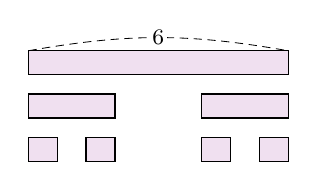
\begin{tikzpicture}[scale=0.55, line width=0.5pt]
  \draw[fill=violet!12] (0,2) rectangle (6,2.55);
  \draw[fill=violet!12] (0,1) rectangle (2,1.55);
  \draw[fill=violet!12] (4,1) rectangle (6,1.55);
  \draw[fill=violet!12] (0,0) rectangle (0.667,0.55);
  \draw[fill=violet!12] (1.333,0) rectangle (2,0.55);
  \draw[fill=violet!12] (4,0) rectangle (4.667,0.55);
  \draw[fill=violet!12] (5.333,0) rectangle (6,0.55);
  \draw[densely dashed, line width=0.3pt] (0,2.55)
    to[bend left=10] node[midway, fill=white, inner sep=1pt, font=\footnotesize] {$6$} (6,2.55);
\end{tikzpicture}
}\end{minipage}\par
